\documentclass[12pt]{article}
\usepackage{amsmath}
\usepackage{graphicx}
\usepackage{hyperref}
\usepackage{circuitikz}
\usetikzlibrary{arrows,shapes,calc,positioning}


\title{Electrical Applications - Transformer}
\author{Nicholas Martinez}
\date{03/13/19}
\begin{document}
	
\maketitle
	
\begin{abstract}
	In this final project, we will explore the physics behind a critical device that allows us to harness the massive amounts of power distributed by the electrical grid system, namely the \textit{transformer}. Starting with a cross sectional analysis of the various components of a transformer, we will cover extensively the physics behind stepping down voltage to use usable level. We will also take a look at some interesting questions behind transformers that can be observed on a day to day basis, such as why do transformers hum/vibrate, and what exactly makes a transformer explode during a heavy storm. 
	
\end{abstract} 

\section{Introduction}

\paragraph{Modern Electrical Applications - The Transformer}

Of the many revolutionary discoveries of humanity, the discovery and following applications of electricity and the electromagnetic laws, without hesitation ranks itself among the topmost pinnacles of human achievement, completely transforming our world into the modern era as we know it today. Beginning with the simple application of illuminating a room with a light bulb around a simple circuit, we now enjoy the luxury of fully electrified housing units with the ability to tap into the electrical grid system simply by plugging in to a wall socket unit. And while the electrical grid system as a whole is a modern marvel in itself, the scope of this article could not even begin to cover the full complexities of how a mega system like a communal power grid is engineered. Instead we will take a look into one of the most critical elements to delivering usable and practical electricity to our homes. 

This device is known as a \textit{transformer}, and it is the primary reason that we are able enjoy the use of small scale electronic devices within the household, while also drawing from a power source of incredible energy that unfiltered would destroy any small electrical device connected to it. Simply stated, a transformer is a static electrical device that when supplied an electrical current input, is able to increase or decrease the input voltage and output a different voltage, also known as \textit{stepping up} or \textit{stepping down} voltage. 

Transformers tend to be especially known when they occasionally explode, causing a bright blue flash of light that can be seen for miles from the source. Likewise, pedestrians often notice transformers when they can make an significant 'buzzing' noise. Both of these phenomena are directly related to the internal structure and physical laws governing the operation of these devices.

\section{History}

\paragraph{Conceptual Origins - Induction} 
The core principle that governs the operations of an electrical transformer is the concept of \textit{electromagnetic induction}. The discovery of mutual magnetic induction between two coupled circuits is credited to the English physicist and chemist Micheal Faraday (1791-1867).

Although Faraday never possessed a formal education, he began working as an assistant at the Royal Institution under the chemist Humphrey Davy at only 21 years old, in which he was able to conduct a number of experiments regarding electromagnetism. From his initial experiments on iron filings and their response to magnets, he coined the term \textit{line of force} to describe the movements of the filings when exposed to a magnet. This eventually evolved into discovering mutual magnetic induction by noting a current induced on one coil wound on a toroidal iron core when the current on another coil also wound on the core was rapidly fluctuated. 

Furthering this experiment, he also observed a current induced on such coils when a magnet was placed and moved inside the space within the core of the wound coils. Faraday then was able to describe this phenomena and coined the term as the \textit{electromotive force}. This eventually culminated into what is now known as \textit{Faraday's law of induction}, described by the below equation. 

\begin{center}
\begin{huge}
	\fbox{
	\vspace{5mm}
	$\mid{\varepsilon}\mid \hspace{2mm }= \left|{{\mathrm{d}\Phi_\text{B}} \over \mathrm{d}t}\right|$
 	\vspace{5mm}	
}
\end{huge}
\end{center}

Where $\mid{\varepsilon}\mid$ is the magnitude of the electromagnetic force in volts, and $\Phi_\text{B}$ is the magnetic flux through the circuit. This equation is reflexive in the sense that the electromagnetic force is induced by the magnetic flux that is produced by some electromagnetic force. This property of electromagnetism will be discussed more in depth in the following section.


Though what Faraday had missed in his description of the electromotive force in his experiments on toroidal coils wound on an iron core is the special relationship between the two coils and how many turns ( or how many times it is wrapped around ) each coil possessed. This was later discovered in 1836 by Reverend Nicholas Callan (1799 - 1864). Inspired by Faraday, Callan had sought out a method to generate a higher voltage of electricity than what was currently available at the time. Similar to the experiments done by Faraday, Callan began constructing what is now known as an inductor coil, or a spark coil. By taking an iron bar and wrapping two coils around it, connecting the beginning of each coil to each other. When he had then connected a battery to the winding end of one coil, he noticed that upon disconnecting the battery terminals from the wire, a spark resulted at the end of the two coils.

Through further experiments, Callan was able to increase the intensity of the resultant spark by increasing the size of the secondary coil, while using a battery of the same voltage. Callan had effectively created the first induction transformer, and had also created a practical demonstration of Lenz's law.

\begin{center}
	\begin{huge}
		\fbox{
		\vspace{5mm}
		${\varepsilon} \hspace{2mm }= -{{\partial\Phi_\text{B}} \over \partial t}$
		\vspace{5mm}	
	}
	\end{huge}
\end{center}


\section{Induction Coils}
\paragraph{Callan's Coil Explained} 
The induction coil Callan had created in his experiments laid the beginning conceptual blueprints for the eventual engineering of the modern day transformer. 

\begin{center}
\begin{circuitikz} \draw
	(0,0) to[switch] (-2,0)
	to[battery] (-4,0)
	to[] (-4, 2)
	to[american inductor] (2, 2)
	to[] (2,0)
	to[capacitor] (3,0)
	to[] (3,-2)
	to[] (0,-2)
	to[] (0,0);
	\draw (3,0)
	to[short,*-] (3,2)
	to[short,-*	] (2,2);
	\draw (1,2) to[short,*-] (1,4)
	to[short,-*] (-1,4);
	
	\draw (-2,4) to[short,*-] (-4,4)
	to[short,-*] (-4,2);
	\draw[dashed] (-2,2.5) to[] (0,2.5)
	to[] (0,1.7) 
	to[] (-2,1.7)
	to[] (-2,2.5);
	\draw (-1.7,2.3) to[] (-.3,2.3);	
	\draw (-1.7,2.4) to[] (-.3,2.4);	
	
\end{circuitikz}
\end{center}

Above we have an electrical diagram for an inductor coil. As we know from Faraday's law of induction, the electromotive force generates a magnetic flux directly proportional to the current flowing through the inductor, and with Len'z law we see that this flux is proportionally opposed to that current when $\mathbf{t=0}$ ( at the moment the switch is closed ) by creating a voltage difference at the poles of the inductor, which reduces as the electromagnetic field stops expanding. As soon as this point is reached, the current passing through the inductor will reach its maximum value after $\mathbf{5T}$, or 5 time constants, where T is

\begin{center}
	\begin{huge}
		\fbox{
		\vspace{5mm}
		$\mathbf{T = \frac{L}{R}}$
		\vspace{5mm}	
		}
	\end{huge}
\end{center}
\noindent
\begin{center}
	
Where $\mathbf{L}$ = Inductance of the coil \break
Where $\mathbf{R}$ = Total resistance of the circuit 
\end{center}
\begin{center}
\begin{LARGE}
	\fbox{
		$\mathbf{L} = \frac{N^2 \mu A}{l}$
	}\end {LARGE}
\end{center}
Above is the formula for the Inductance of a Coil from which we can derive using Lenz's Law. 

\begin{center}
	\begin{LARGE}
	${\varepsilon} \hspace{2mm }= -{{\partial\Phi_\text{B}} \over \partial t}$	\end{LARGE}\\
	\vspace{5mm}
	For a fixed area and changing current, Faraday's law becomes\\
	\vspace{5mm}
	\begin{LARGE}
		${\varepsilon} \hspace{2mm }= -A{{\partial B} \over \partial t}$
	\end{LARGE}\\
	\vspace{5mm}
	For the magnetic field of a coil becomes\\
	\vspace{5mm}
	\begin{LARGE}
		${B} = {\hspace{2mm } \mu{N} \over L} I$
	\end{LARGE}\\
	\vspace{5mm}
	Which the \textit{emf} is then approximated by\\
	\vspace{5mm}
	\begin{LARGE}
		${\varepsilon} = {\hspace{2mm } \mu{N^2} \over L} \hspace{2mm}{{\partial I} \over \partial t}$
	\end{LARGE}\\
	\vspace{5mm}
	Using inductance from Faraday's Law\\
	\vspace{5mm}
	\begin{LARGE}
		${\varepsilon} \hspace{2mm }= -L{{dI} \over dt}$
	\end{LARGE}\\
	\vspace{5mm}
We arrive at\\
\vspace{5mm}
\begin{center}
	\begin{LARGE}
		\fbox{
			$\mathbf{L} = \frac{N^2 \mu A}{l}$
		}\end {LARGE}
	\end{center}
\end{center} 

Going back to Callan's discovery of increased spark voltage based on the amount of wraps in the coil (${N}$), and the larger area of the coil (${A}$) , combined with the magnetic permeability  (${\mu}$),  which in this case Callan used iron, through these equations we can see that by increasing the area and wraps of the coil, Callan had created an inductor with higher \textit{inductance}, measured in the units of \textit{Henry} (${H}$). 

	\begin{center}
		From Faraday's law we can see how inductance relates to voltage as the current diminishes over time\\
		\vspace{5mm}
		\begin{LARGE}
			\fbox{
				$\mathbf{L} = \frac{V}{\frac{A}{t}}$
			}\end {LARGE}
	\end{center}

As the inductance of an inductor rises, the voltage must necessarily increase while the amperage decreases. Thus by giving an input voltage to an inductor with high inductance, the magnetic field generated as the result of that voltage is dependent on the inductance and stores energy in that magnetic field to a maximum point until the current stabilizes and the resistance from the inductor reaches 0. Though as soon as the source of current is removed, as when Callan removed the battery terminals from the circuit, or in the case of the above diagram, the switch is open, the high amount of energy stored in the induced magnetic field dependent on the inductance of the inductor is converted into voltage, which based on the inductance will be of much greater voltage than was initially supplied to the inductor in the first place!
Thus the physics of inductance acts as a step up transformer in this case. 

\begin{center}
	\begin{circuitikz} \draw
		(0,0) to[switch] (-2,0)
		to[battery] (-4,0)
		to[] (-4, 2)
		to[american inductor] (2, 2)
		to[] (2,0)
		to[capacitor] (3,0)
		to[] (3,-2)
		to[] (0,-2)
		to[] (0,0);
		\draw (3,0)
		to[short,*-] (3,2)
		to[short,-*	] (2,2);
		\draw (1,2) to[short,*-] (1,4)
		to[short,-*] (-1,4);
		
		\draw (-2,4) to[short,*-] (-4,4)
		to[short,-*] (-4,2);
		\draw[dashed] (-2,2.5) to[] (0,2.5)
		to[] (0,1.7) 
		to[] (-2,1.7)
		to[] (-2,2.5);
		\draw (-1.7,2.3) to[] (-.3,2.3);	
		\draw (-1.7,2.4) to[] (-.3,2.4);	
		
	\end{circuitikz}
\end{center}
One thing to note before moving on to the next section is that in our diagram above, there is a capacitor facing the inductor and the switch. The reason for this capacitor is because when the energy is released from the rapidly collapsing magnetic field around the inductor, the electrons travel in both directions, which in one ( the initial direction of electrons flowing ) creates the spark across the air gap, or in Callan's case where the beginning of the coils of the inductor met, and the other ( the voltage that was resiting the change in the current which induced it ), also known the \textit{counter-electromotive force}, would end up burning out the terminals of the battery if there were no other route for it to take. With the capacitor in parallel to the battery, the counter-electromotive force instead is stored in the capacitor. 


\section{Transformers}
\paragraph{From the Induction Coil to the Modern Transformer} As we have just discovered in the previous section, the first induction coil ( a type of transformer ) laid the conceptual groundwork for creating a transformer that can both step up and step down voltage. Though one thing to note is that Callan's inductor coil operated only on direct current ( DC current ). Since nearly all standard household electric devices operate on alternating current ( AC current ), the type of every day transformer used in electric grid applications is engineered with this in mind. 

Though we already have the two electromagnetic laws that make these devices possible, and the core concepts in an AC step down transformer are very similar to Callan's inductor coil, there are some major differences in the design. The key in creating a modern transformer relies on the inductance relationship between \textit{two} inducting coils, and is critically dependent on an alternating current. Lets reexamine Faraday's law of induction that we introduced in Section 2.  

\begin{center}
	\begin{huge}
		\fbox{
			\vspace{5mm}
			$\mid{\varepsilon}\mid \hspace{2mm }= \left|{{\mathrm{d}\Phi_\text{B}} \over \mathrm{d}t}\right|$
			\vspace{5mm}	
		}
	\end{huge}
\end{center}
\vspace{5mm}	
When it was stated earlier that this equation is in a sense reflexive, we are referring directly to the functionality of a modern transformer. 
\vspace{5mm}	
\begin{center}
\begin{circuitikz} \draw
	(0,0) node[transformer] (T) {}
	(T.A1) node[anchor=east] {}
	(T.A2) node[anchor=east] {}
	(T.B1) node[anchor=west] {}
	(T.B2) node[anchor=west] {}
;

\draw[-latex] (-4,-1) -- (-1.5,-1) node[below] {$12kV$};
\draw[-latex] (1,-1) -- (3.5,-1) node[below] {$120V$};
		\draw[dashed] (-.7,-2.5) to[] (.7,-2.5)
to[] (.7,.5) 
to[] (-.7,.5)
to[] (-.7,-2.5);
\end{circuitikz}
\end{center}
\vspace{5mm}	
In this very basic diagram of a modern transformer, we have an input voltage of ${12V}$ going through the primary inductor coil on the left. From Faraday's law we see this creates a magnetic field with magnitude proportional to that voltage.

We also see our iron core, represented by the dashed lines looping around the primary and secondary inductor coils. 
\vspace{5mm}
\begin{center}
	\begin{LARGE}
		\fbox{
			$\mathbf{L} = \frac{N^2 \mu A}{l}$
		}\end {LARGE}
	\end{center}
\vspace{5mm}
Back in our derivation of the inductance formula from Lenz's law and Faraday's law, we see that the magnetic permeability ${\mu}$ is related to the units of induction of the inductor. Iron has a particularly high level of magnetic permeability, and thus the primary coil is ability to induct that magnetic field through the looping iron core and reach the secondary coil on the right. 

We now can use the reflexive property of Faraday's law of induction where 
\vspace{5mm}
\begin{center}
	\begin{huge}
		\fbox{
			\vspace{5mm}
			$\mid{\varepsilon}\mid \hspace{2mm }= \left|{{\mathrm{d}\Phi_\text{B}} \over \mathrm{d}t}\right|$
			\vspace{5mm}
			\hspace{5mm}
			$\Longleftrightarrow$
			\hspace{5mm}
						\vspace{5mm}
					
			$	\left|{{\mathrm{d}\Phi_\text{B}} \over \mathrm{d}t}\right|=\mid{\varepsilon}\mid \hspace{2mm } $
			\vspace{5mm}	
		}
	\end{huge}
\end{center}
\vspace{5mm}
What this is saying is that from the magnetic flux created by the primary coils input voltage can then be converted back into voltage on the secondary coil. So through the principles of inductance through an inducting material, we are able to transfer an arbitrary voltage. Though we need one more equation to be able to successfully step up and step down voltage through each inductor. 

As we have mentioned before in Callan's induction coil, the magnitude of inductance is proportional to the strength of the induced magnetic field, which is also proportional to the voltage difference created from the generation of the magnetic field. By transitivity this necessarily implies that inductance has a direct effect on the voltage generated. And while our magnetic permeability remains constant to the material of the iron core and the copper wiring, we can change the number of turns of each coil to change its inductance and thus change the voltage that coil generates.

For that we have 
\vspace{5mm}
\begin{center}
	\begin{LARGE}
		\fbox{
			$\frac{V_s}{V_p} = \frac{N_s}{N_p}$
		}\end {LARGE}
	\end{center}
	\vspace{0mm}
	\noindent
	\begin{center}
		Where $\mathbf{V}_p = \mathbf{Voltage}_{primary}$\linebreak
		Where $\mathbf{V}_s = \mathbf{Voltage}_{secondary}$\linebreak
		Where $\mathbf{N}_p = \mathbf{Turns}_{primary}$\linebreak
		Where $\mathbf{N}_s = \mathbf{Turns}_{secondary}$\linebreak
	\end{center}

What this means in relation to our transformer is that the relationship between the number of turns on each coil is proportional to the relationship between the input and output voltage. 
\vspace{5mm}	
\begin{center}
	\begin{circuitikz} \draw
		(0,0) node[transformer] (T) {}
		(T.A1) node[anchor=east] {primary}
		(T.A2) node[anchor=east] {}
		(T.B1) node[anchor=west] {secondary}
		(T.B2) node[anchor=west] {}
		;
		
		\draw[-latex] (-4,-1) -- (-1.5,-1) node[below] {$12V$};
		\draw[-latex] (1,-1) -- (3.5,-1) node[below] {$12V$};
		\draw[dashed] (-.7,-2.5) to[] (.7,-2.5)
		to[] (.7,.5) 
		to[] (-.7,.5)
		to[] (-.7,-2.5);
	\end{circuitikz}
\end{center}
\vspace{5mm}

In this example we have a ${12V}$ input on the primary coil, and a ${12V}$ output on the secondary coil. Plugging this into our transformer equation
\vspace{5mm}
\begin{center}
	\begin{LARGE}

			$(\frac{V_s}{V_p} = \frac{N_s}{N_p}) \rightarrow ({V_s}{N_p} = {N_s}{V_p})$\\
			\vspace{1mm}
			$\downarrow$\\
			\vspace{1mm}
			$({V_s}{N_p} = {N_s}{V_p}) \rightarrow ({12N_p} = {12N_s})$\\
			\vspace{1mm}
			$\downarrow$\\
			\vspace{1mm}
			$({12N_p} = {12N_s}) \rightarrow ({N_p} = {N_s})$\\
			\vspace{1mm}
			$\downarrow$\\
			\vspace{1mm}
	
		\fbox{${N_p} = {N_s}$}
			\end {LARGE}
	\end{center}
	\vspace{5mm}
	Meaning for a 1:1 voltage ratio from input voltage to output voltage, the two induction coils must have the same number of turns. If we apply the same formula to our previous diagram that steps down ${12kV} \rightarrow {120V}$
	
	\vspace{5mm}	
	\begin{center}
		\begin{circuitikz} \draw
			(0,0) node[transformer] (T) {}
			(T.A1) node[anchor=east] {primary}
			(T.A2) node[anchor=east] {}
			(T.B1) node[anchor=west] {secondary}
			(T.B2) node[anchor=west] {}
			;
			
			\draw[-latex] (-4,-1) -- (-1.8,-1) node[below] {$120000V$};
			\draw[-latex] (1,-1) -- (3.5,-1) node[below] {$120V$};
			\draw[dashed] (-.7,-2.5) to[] (.7,-2.5)
			to[] (.7,.5) 
			to[] (-.7,.5)
			to[] (-.7,-2.5);
		\end{circuitikz}
	\end{center}
	\vspace{1mm}
	\begin{center}
		\begin{LARGE}
			
			$(\frac{V_s}{V_p} = \frac{N_s}{N_p}) \rightarrow ({V_s}{N_p} = {N_s}{V_p})$\\
			\vspace{1mm}
			$\downarrow$\\
			\vspace{1mm}
			$({V_s}{N_p} = {N_s}{V_p}) \rightarrow ({120N_p} = {120000N_s})$\\
			\vspace{1mm}
			$\downarrow$\\
			\vspace{1mm}
			$({120N_p} = {120000N_s}) \rightarrow ({N_p} = {1000N_s})$\\
			\vspace{1mm}
			$\downarrow$\\
			\vspace{1mm}
			$({N_p} = {1000N_s}) \rightarrow (\frac{N_s}{N_p} = \frac{1}{1000})$\\
			$\downarrow$\\
			\vspace{1mm}
			\fbox{$\frac{N_s}{N_p} = \frac{1}{1000}$}
			\end {LARGE}
		\end{center}
		\vspace{5mm}
We find that the primary coil has 1000 times as many turns as the secondary coil. So if our secondary coil consists of 20 turns, then our primary coil must have 20,000 turns. 


\paragraph{Alternating Current} Though we are close, we are missing the final description of the laws of inductance that let us understand why Callan's coil operated only on DC voltage while the modern transformer operates only on AC voltage. 

Recall from Faraday's law of induction
			\vspace{5mm}
\begin{center}
	\begin{huge}
		\fbox{
			\vspace{5mm}
			$\mid{\varepsilon}\mid \hspace{2mm }= \left|{{\mathrm{d}\Phi_\text{B}} \over \mathrm{d}t}\right|$
			\vspace{5mm}	
		}
	\end{huge}
\end{center}
			\vspace{5mm}
Which states that the voltage generated is directly proportional to the magnitude of magnetic flux with respect to time. What this is saying is that the voltage potential is only realized during a change in magnetic flux, which is the result from a change in current. Recall in Callan's Inductor coil that he was only able to generate the high voltage spark as soon as he disconnected the terminals of the battery from the inductor.

This is because after the inductor has passed $\mathbf{5T}$, the current reaches its maximum value, drops its opposing resistance to the current ( Lenz's Law ) and the magnetic field stabilizes as an expression of the voltage passed to it from initial contact with the battery ( storing energy in the magnetic field ). Though as soon as the current changes, which happens when the battery is disconnected from the coils, the magnetic field experiences the changing flux in reverse, essentially collapses on itself, and converts all of the stored energy in it's induced magnetic field, back to voltage. Except that based on the inductance of the coil, the voltage will necessarily be higher than the initial voltage supplied. That voltage travels through each coil and jumps the air gap between the coils where the battery terminals used to stand. 
\vspace{5mm}
	\begin{center}
	\begin{circuitikz} \draw
		(0,0) node[transformer] (T) {}
		(T.A1) node[anchor=east] {primary}
		(T.A2) node[anchor=east] {}
		(T.B1) node[anchor=west] {secondary}
		(T.B2) node[anchor=west] {}
		;
		
		\draw[-latex] (-4,-1) -- (-1.8,-1) node[below] {$120000V$};
		\draw[-latex] (1,-1) -- (3.5,-1) node[below] {$120V$};
		\draw[dashed] (-.7,-2.5) to[] (.7,-2.5)
		to[] (.7,.5) 
		to[] (-.7,.5)
		to[] (-.7,-2.5);
	\end{circuitikz}
\end{center}
Except in the case of our transformer, and especially such a transformer connected to the electric grid, continuously connecting and disconnecting the power source is not feasible. Likewise, creating sparks of over 60,000 Volts over air gaps on each transformer across an urban environment is far too dangerous for sustainable operation. Though if we do not, as soon as the primary inductor coil reaches its maximum magnetic state, no more voltage will be induced in the secondary coil, and thus no current will flow through. 

Instead we must figure out an alternative way to create a continuously varying magnetic flux. And because we know that the magnetic field is intrinsically related to the voltage, if we are able to find a way to continuously modulate the voltage,  we can then keep the magnetic flux going and induct the current across the induction coils.

This is exactly where alternating current comes in. Expressed as a sinusoidal wave of voltage.
\vspace{5mm}\\
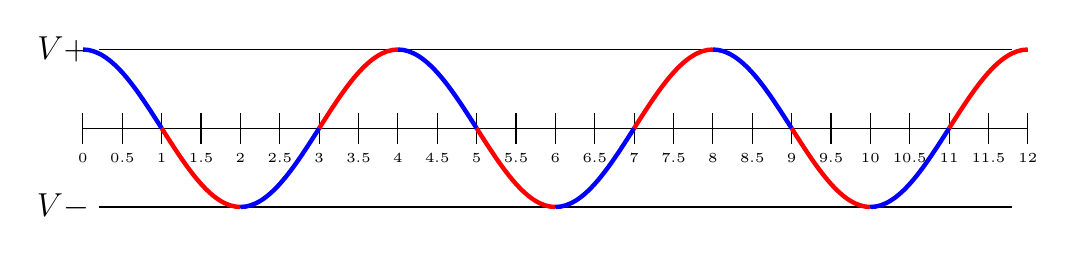
\begin{tikzpicture}
    \draw (0,0) -- (12,0);
\draw (0.2,1)node[left,font=\large] {$V+$} -- (11.8,1);
\draw (0.2,-1)node[left,font=\large] {$V-$} -- (11.8,-1); 
\foreach \x in {0,0.5,...,12}{
	\draw (\x,-0.2)node [below,font=\tiny,] {\x} -- (\x,0.2) ;
}
\draw[ultra thick, blue] (0,1) cos (1,0); 
\draw[ultra thick, red] (1,0) sin (2,-1);    %% the real business in this line
\draw[ultra thick, blue] (2,-1) cos (3,0);    %% the real business in this line
\draw[ultra thick, red] (3,0) sin (4,1);    %% the real business in this line
\draw[ultra thick, blue] (4,1) cos (5,0);    %% the real business in this line
\draw[ultra thick, red] (5,0) sin (6,-1);    %% the real business in this line
\draw[ultra thick, blue] (6,-1) cos (7,0);    %% the real business in this line
\draw[ultra thick, red] (7,0)  sin (8,1);    %% the real business in this line
\draw[ultra thick, blue] (8,1) cos (9,0);    %% the real business in this line
\draw[ultra thick, red] (9,0) sin (10,-1);    %% the real business in this line
\draw[ultra thick, blue] (10,-1) cos (11,0);    %% the real business in this line
\draw[ultra thick, red] (11,0) sin (12,1);    %% the real business in this line
\end{tikzpicture}
\vspace{5mm}\\
Since we know that voltage is proportional to the magnetic field, we can think of this graph as representing both the input voltage to the primary coil, and the state of the magnetic field for the primary coil. 

For the secondary conductor with a lower amount of turns, and thus a lower inductance and a lower output voltage, the secondary coil's graph should look exactly the same except with an amplitude corresponding to the voltage determined by the inductance. 
\vspace{5mm}\\
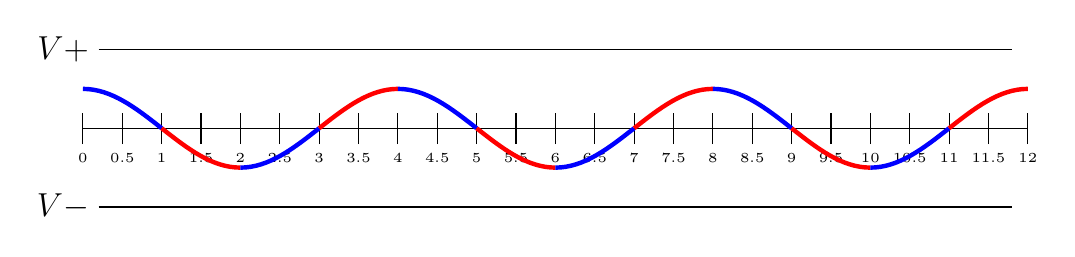
\begin{tikzpicture}
\draw (0,0) -- (12,0);
\draw (0.2,1)node[left,font=\large] {$V+$} -- (11.8,1);
\draw (0.2,-1)node[left,font=\large] {$V-$} -- (11.8,-1); 
\foreach \x in {0,0.5,...,12}{
	\draw (\x,-0.2)node [below,font=\tiny,] {\x} -- (\x,0.2) ;
}
\draw[ultra thick, blue] (0,.5) cos (1,0); 
\draw[ultra thick, red] (1,0) sin (2,-.5);    %% the real business in this line
\draw[ultra thick, blue] (2,-.5) cos (3,0);    %% the real business in this line
\draw[ultra thick, red] (3,0) sin (4,.5);    %% the real business in this line
\draw[ultra thick, blue] (4,.5) cos (5,0);    %% the real business in this line
\draw[ultra thick, red] (5,0) sin (6,-.5);    %% the real business in this line
\draw[ultra thick, blue] (6,-.5) cos (7,0);    %% the real business in this line
\draw[ultra thick, red] (7,0)  sin (8,.5);    %% the real business in this line
\draw[ultra thick, blue] (8,.5) cos (9,0);    %% the real business in this line
\draw[ultra thick, red] (9,0) sin (10,-.5);    %% the real business in this line
\draw[ultra thick, blue] (10,-.5) cos (11,0);    %% the real business in this line
\draw[ultra thick, red] (11,0) sin (12,.5);    %% the real business in this line
\end{tikzpicture}\\




\end{document}
